\section{TinyML and AI on the Edge}
\subsection{Edge computing & AIoT overview}
\indent In recent years, edge computing has emerged as a promising technology with significant potential in various fields. It offers advantages such as reduced latency and cost savings. Unlike traditional cloud computing, edge computing enables data processing at the edge of the network. 
This approach brings data computing closer to the data source, greatly benefiting the development of time-sensitive applications. Additionally, by performing processing locally, edge computing reduces network traffic and minimizes data transmission, resulting in substantial cost savings. [20]

From the advantages of edge computing, integrating edge devices with IoT ecosystems can facilitate the shift of computation from the cloud to the network edge through collaboration among sensors, edge devices, and cloud facilities.
However, edge hardware has limited resources and is platform-dependent, which restricts its ability to support advanced and complex services such as machine learning applications. It obstructs the development of a standardized machine learning framework for all IoT-edge devices.

Furthermore, while existing embedded processors can handle generic sensor data processing and web-based applications, machine learning applications rely on sophisticated hardware chips such as graphics processing units (GPUs). 
These chips demand significant power and memory capacity to execute deep neural network models. Thus, the current landscape challenges achieving the envisioned "cloud-to-embedded" aspect. [21]

\subsubsection{TinyML overview}
\indent  Since 2019, a new technology called TinyML has been addressing the challenges of designing power-efficient deep learning models (in the milliwatt range and below) to be integrated into embedded systems like AIoT/IIoT/IoT devices.
TinyML is defined as follows: “machine learning aware architectures, frameworks, techniques, tools, and approaches which are capable of performing on-device analytics for a variety of sensing modalities (vision, audio, speech, motion, chemical, physical, textual, cognitive) at mW (or below) power range setting, while targeting predominately battery-operated embedded edge devices suitable for implementation at large scale use cases preferable in the IoT or wireless sensor network domain” (TinyML, 2021a). Thus, TinyML can be envisaged as the composition of three key elements (i) software, (ii) hardware, and (iii) algorithms. [25]
\begin{center}
    \begin{figure}[!htp]
        \centering
        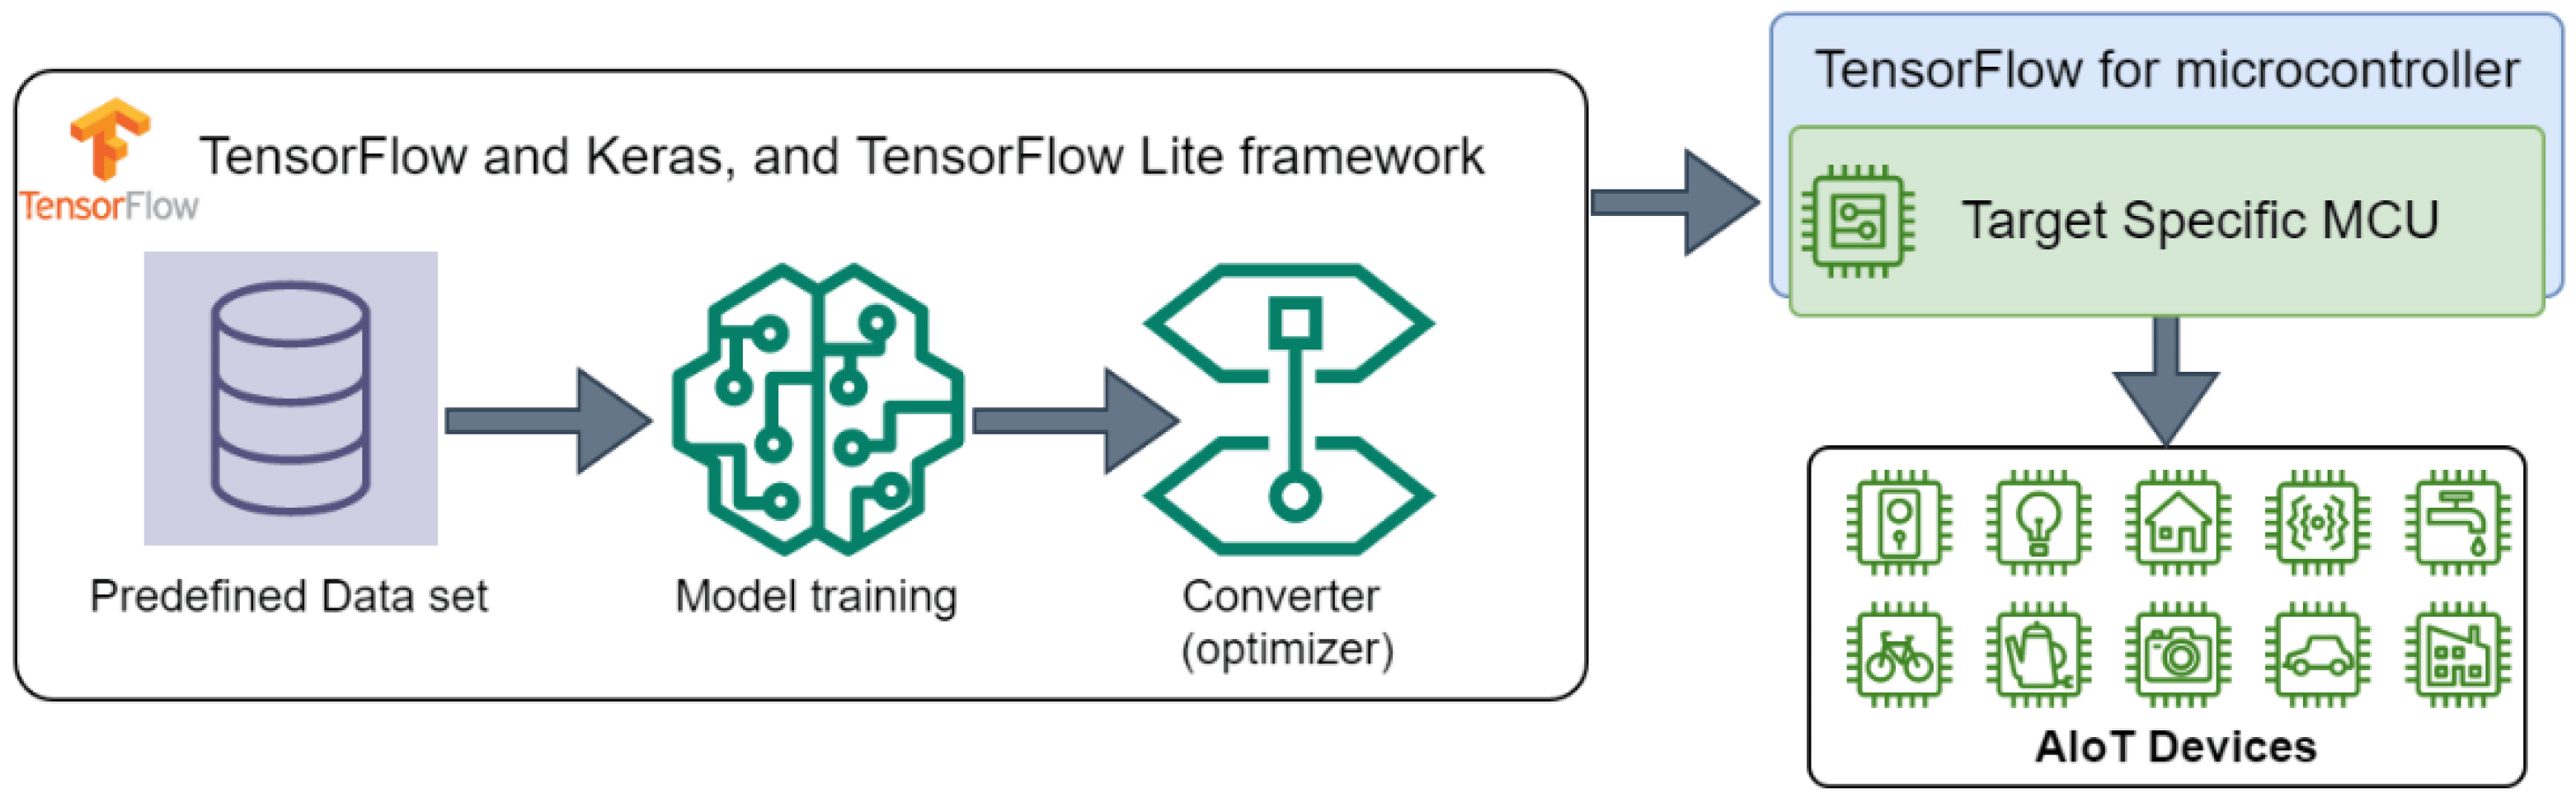
\includegraphics[width=0.8 \textwidth]{image/tf_lite.webp}
        \caption{TensorFlow lite for microcontrollers}
        \label{subsection}
    \end{figure}
    \end{center}

The above figure illustrates the workflow for developing deep learning algorithms. First, the dataset is created based on the chosen neural network model (CNN, RNN, etc.). 
In some cases, dataset preprocessing may be necessary to optimize training and improve performance. Training is typically conducted on a workstation or supercomputer server using frameworks like TensorFlow or PyTorch. 
The trained model's precision is usually float32, and its parameter memory footprint is significant (larger than the available flash and SRAM on a microcontroller unit).

TensorFlow Lite, within the TensorFlow framework, provides a converter to optimize the trained model by reducing the memory footprint and computational power requirement (using int8 instead of float32). [22]
The TensorFlow Lite framework converter takes the trained model (saved in the xx.h5 file) and produces three optimized models: int8 quantization, integer dynamic quantization, and float16. One of these files, such as the int8 quantization tflite file, 
can be utilized in other tools like the X-CUBE-AI [23] extension pack of STM32CubeMx [24]. These tools can generate C codes that can be deployed and run on microcontrollers [22]
\subsection{TinyML framework and software}
\indent TinyML requires several hardware specifications, libraries, and software platforms to leverage predictions. We only focus on software platforms and frameworks for this project's scope.
TinyML frameworks and softwares are being developed to support the deployment of machine learning models on embedded devices. Some of examples are as follows: [23]
\begin{itemize}
    \item TensorFlow Lite for Microcontrollers (TFLite Micro): TensorFlow Lite is a popular ML framework developed by Google. TFLite Micro is a specialized version of TensorFlow Lite designed for microcontrollers and other small devices. It provides a set of tools and libraries for training and deploying ML models on edge devices with limited resources. TFLite Micro supports various hardware platforms and offers optimizations for memory and computational efficiency.
    \item Edge Impulse: Edge Impulse is an end-to-end platform for building and deploying TinyML applications. It provides a comprehensive workflow for collecting, preprocessing, training, and deploying ML models on edge devices. Edge Impulse supports a wide range of sensors and development boards, making it accessible for developers without extensive ML expertise. It also offers integration with popular ML frameworks like TensorFlow and Keras.
    \item uTensor: uTensor is an open-source ML inference library specifically designed for microcontrollers. It allows developers to deploy trained ML models on resource-constrained devices with minimal code overhead. uTensor provides a C++ API for loading and executing models and supports quantization techniques to reduce model size and improve inference speed. It also offers compatibility with TensorFlow and supports various microcontroller platforms.
    \item μTVM (pronounced "micro TVM") is a framework that extends the TVM (Tensor Virtual Machine) deep learning compiler and runtime to support edge devices. μTVM supports quantization techniques, such as reduced-precision arithmetic, to reduce the memory footprint and improve inference speed while maintaining acceptable accuracy levels. It also offers support for other features, such as hardware abstraction (to support different microcontroller platforms) and model compression (to reduce the size of the model).
\end{itemize}

\subsection{Conclusion}
\indent The Edge-IoT ecosystem holds immense potential in leveraging intelligent decision-making capabilities at the network edge. The integration of machine learning into resource-limited embedded devices has emerged as a crucial requirement for future-oriented applications. 
Therefore, a thorough exploration of the TinyML paradigm is essential to advance the current landscape of edge-aware machine learning.
